\chapter{Quickstart}
\label{chapter:quickstart}


\chapterDescription
  {
    Should take you around 15 minutes to get the
    code up and running. Then another 15 minutes to have the first static
    adaptive Cartesian grid.
  }
  {
    No previous knowledge, but some experience with the Linux
    command line and Paraview is advantageous.
  }



\section{Download and install}

To start work with Peano, you need at least two things.

\begin{enumerate}
  \item The Peano source code. Today, the source code consists of two important
  directories. The \texttt{peano} directory holds the actual Peano code. An
  additional \texttt{tarch} directory holds Peano's technical architecture.
  \item The Peano Development Toolkit (PDT). The PDT is a small Java archive. It
  takes away the cumbersome work to write lots of glue code, i.e.~empty
  interface implementations, default routines, \ldots, so we use it quite
  frequently.
\end{enumerate}

\noindent
For advanced features, you might want to use some {\bf toolboxes}.
A toolbox in Peano is a small collection of files that you store in a directory
and adopt all pathes accordingly.
From a user's point of view, when we use the term toolbox we actually mean this
directory with all its content.



\begin{remark}
Originally, we hoped that Peano's technical architecture (\texttt{tarch}) might
become of value for several projects, i.e.~projects appreciate that they do not
have to re-develop things such as logging, writing of output files, writing
support for OpenMP and TBB, and so forth.
To the best of our knowledge, the tarch however is not really used by someone
else, so we cannot really claim that it is independent of Peano.
Nevertheless, we try to keep it separate and not to add anyting AMR or
grid-specific to the tarch.
\end{remark}

There are two ways to get hold of Peano's sources and tools. You either {\em
download the archives from the website} or you {\em access the repository
directly}.
Both variants are fine.
We recommend to access the respository directly.


\subsection{Download the archives from the website}

If you don't want to download Peano's whole archive, change to Peano's webpage
\url{http://www.peano-framework.org} and grab the files
\begin{itemize}
  \item \texttt{peano.tar.gz} and
  \item \texttt{pdt.jar}
\end{itemize}
from there. If you do so, please skip the first two lines from the script
before. Otherwise, load down the important files with \texttt{wget}. 
Independent of which variant you follow, please unpack the \texttt{peano.tar.gz}
archive. 
It holds all required C++ sources.

\begin{code}
> wget http://sourceforge.net/projects/peano/files/peano.tar.gz
> wget http://sourceforge.net/projects/peano/files/pdt.jar
> tar -xzvf peano.tar.gz
\end{code}


\noindent
There's a couple of helper files that we use IN the
cookbook. 
They are not necessarily required for each Peano project, but for our examples
here they are very useful.
So, please create an additional directory \texttt{usrtemplates} and grap
these files

\begin{code}
> mkdir usrtemplates
> cd usrtemplates
> wget http://sourceforge.net/projects/peano/files/ \
  usrtemplates/VTKMultilevelGridVisualiserImplementation.template 
> wget http://sourceforge.net/projects/peano/files/ \
  usrtemplates/VTKMultilevelGridVisualiserHeader.template 
> wget http://sourceforge.net/projects/peano/files/ \
  usrtemplates/VTKGridVisualiserImplementation.template 
> wget http://sourceforge.net/projects/peano/files/ \
  usrtemplates/VTKGridVisualiserHeader.template 
> wget http://sourceforge.net/projects/peano/files/ \
  usrtemplates/VTK2dTreeVisualiserImplementation.template 
> wget http://sourceforge.net/projects/peano/files/ \
  usrtemplates/VTK2dTreeVisualiserHeader.template 
\end{code}


\begin{remark}
 Many features of Peano are archives into toolboxes, i.e.~small extensions of
 the kernel that simplify your life and provide certain features (such as
 default load balancing or support of patches or particles in the grid). These
 toolboxes are stored in Peano's repository as tar.gz files. Alternatively, you
 can download them from the webpage with \linebreak
 \texttt{wget http://sourceforge.net/projects/peano/files/toolboxes}. 
\end{remark}


\subsection{Access the repository directly}

Instead of a manual download, you might also decide to download a copy of the
whole Peano repository. 
This also has the advantage that you can do a simple \texttt{svn update} anytime
later throughout your development to immediately obtain all kernel
modifications.


\begin{code}
> svn checkout http://svn.code.sf.net/p/peano/code/trunk peano
\end{code}

\noindent
Your directory structure will be slightly different than in the example above,
but this way you can be sure you grabbed everything that has been released for
Peano through the webpage ever.

The archive \texttt{pdt.jar} will be contained in \texttt{pdt}, while the two
source folders will be held by \texttt{src}.
The directory \texttt{usrtemplates} is contained in \texttt{pdt}.


\subsection{Prepare your own project}


From hereon, we recommend that you do not make any changes within Peano
repositories but use your own directory \texttt{peano-projects} for your own
projects.
We refer to one of these projects generically from hereon as \texttt{myproject}.
Within \texttt{peano-projects}, we will need to access the directories
\texttt{peano} and \texttt{tarch}.
It is most convenient to create symbolic links to these files.
Alternatively, you also might want to copy files around or adopt makefiles,
scripts, and so forth.
I'm too lazy to do so and rely on OS links.


\begin{code}
> mkdir peano-projects
> cd peano-projects
> ln -s <mypath>/peano peano
> ln -s <mypath>/tarch tarch
> ls
  peano   tarch
\end{code}




\section{Create an empty Peano project}

Peano projects require four files from the very beginning:

\begin{itemize}
  \item A {\bf specification} file is kind of the central point of contact. It
  defines which data models are used and which operations (algorithmic phases)
  do exist in your project. And it also specifies the project name, namespace,
  and so forth.
  \item A {\bf vertex definition} file specifies which data is assigned to
  vertices in your grid.
  \item A {\bf cell definition} file specifies which data is assigned to
  cells in your grid.
  \item A {\bf state definition} file specifies which data is held in your
  solver globally.
\end{itemize}


\noindent
We will use these files and modify them all the time. For our first step, they
are basically empty.
As mentioned before, we suggest to have one directory per project.
Rather than creating the files as well as the directory manually, we can use the
PDT for this:

\begin{code}
> java -jar <mypath>/pdt.jar  --create-project myproject myproject 
> ls
  myproject  peano  tarch
\end{code}

\noindent
If you are interested in the semantics of the magic arguments, call jar file
without any argument and you will obtain a brief description.
A quick check shows that the aforementioned four files now have been created:


\begin{code}
> ls -al myproject
drwxr-xr-x 2 ...  .
drwxr-xr-x 5 ...  ..
-rw-r--r-- 1 ...  Cell.def
-rw-r--r-- 1 ...  project.peano-specification
-rw-r--r-- 1 ...  State.def
-rw-r--r-- 1 ...  Vertex.def
\end{code}

\noindent
The PDT typically is used only once with the \texttt{--create-project} argument.
From hereon, it serves different purposes. 
That is \ldots




\section{A first spacetree code}

\ldots it helps us to write all the type of code parts that we don't want to
write: {\bf glue code} that does nothing besides gluing the different parts of
Peano together.

We postpone a discussion of the content of the generated files to Chapter
\ref{chapter:basics-explained} and continue to run a first AMR example.
For this, we call the PDT again.
However, this time, we use the generated specification file as input and tell
the tool to create all glue code.


\begin{code}
> java -jar <mypath>/pdt.jar --generate-gluecode \
  myproject/project.peano-specification myproject \
  <mypath>/usrtemplates
\end{code}

\noindent
By default, the autogenerated, (almost) empty four files require the
\texttt{usrtemplates}.
We reiterate that many projects later won't need them.
If we again study the content of our directory, we see that lots of files have
been generated.
For the time being, the \texttt{makefile} is subject of our interest.
Depending on your compiler, you should be able to call \texttt{make} straight
away. 
If it doesn't work, open your favourite text editor and adopt the makefile
accordingly.
\begin{code}
> ls myproject
  adapters   Cell.cpp              Cell.def      
  Cell.h     dastgen               main.cpp     
  makefile   mappings              project.peano-specification  
  records    repositories          runners 
  State.cpp  State.def             State.h
  tests      Vertex.cpp            Vertex.def    
  Vertex.h   VertexOperations.cpp  VertexOperations.h
> make -f myproject/makefile
> ls
  files.mk  myproject  peano  peano-YourProjectName-debug  tarch
\end{code}


\noindent
There it is: the first Peano executable. We can run it straight away:
\begin{code}
> ./peano-YourProjectName-debug
> ls
  files.mk                     grid-0.vtk  myproject  peano  
  peano-YourProjectName-debug  tarch
\end{code}

\noindent
We see that it has produced a vtk file. So it is time to startup Paraview or
VisIt and see what is inside.

\begin{center}
  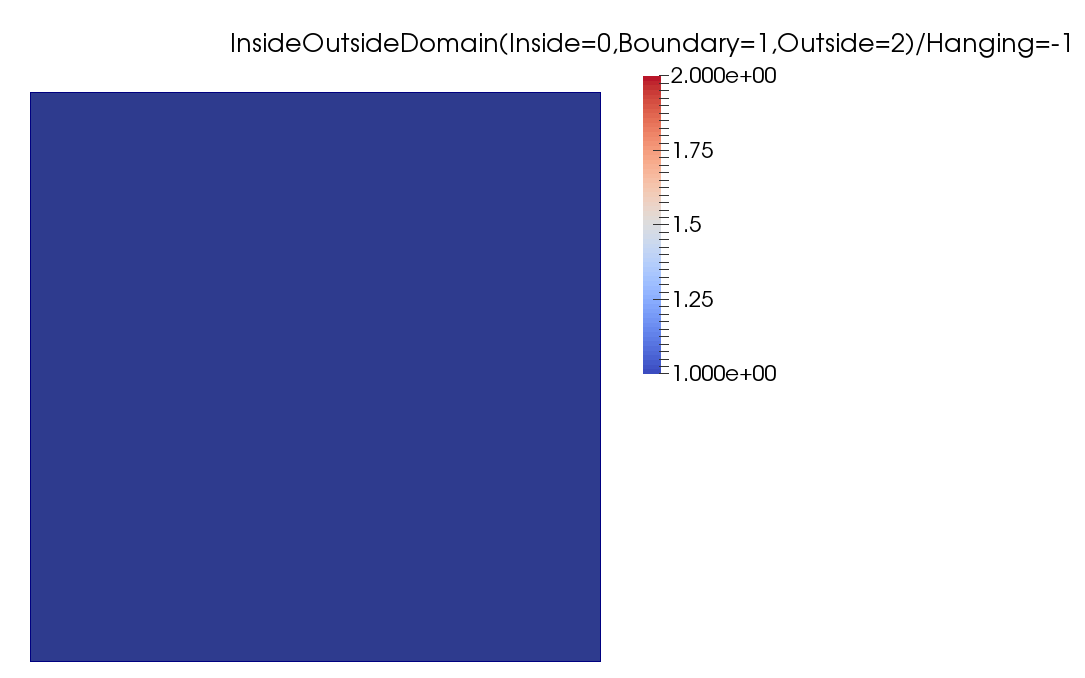
\includegraphics[width=0.8\textwidth]{2_quickstart/screenshot00.png}
\end{center}

\noindent
Congratulations: We have created the simplest adaptive Cartesian grid in 2d that
does exist. A single square!


\section{Some real AMR}

We now set up something slightly more complicated. 
First of all, we switch to a 3d setup rather than 2d. 
For this, open the makefile (\texttt{myproject/makefile}) and alter the
content of the \texttt{DIM} variable.

\begin{code}
# Set Dimension
# -------------
#DIM=-DDim2
DIM=-DDim3
#DIM=-DDim4
\end{code}

\noindent
If you clean your project (\texttt{make -f myproject/makefile clean}) and
rebuild your code, you see that the individual files are translated with the
compile switch 

\begin{code}
g++ ... -DDim3 ....
\end{code}

\noindent
Indeed, this is all that's required for Peano to run a 3d experiment rather than
a 2d setup. 

\begin{remark}
We do support currently up to 10-dimensional setups. If you require higher
dimensions, you might even be able to extend Peano accordingly by changing
solely the file \texttt{peano/utils/Dimensions.h}. But have fun with your memory
requirements exploding.
\end{remark}


Next, we will edit the file \texttt{myproject/mappings/CreateGrid.cpp}. 
Open it with your favourite text editor and search for the operation
\texttt{createBoundaryVertex}. 
Change it into the code below:


\begin{code}
void myproject::mappings::CreateGrid::createBoundaryVertex(
 myproject::Vertex&                          fineGridVertex,
 const tarch::la::Vector<DIMENSIONS,double>& fineGridX,
 const tarch::la::Vector<DIMENSIONS,double>& fineGridH,
 myproject::Vertex * const                   coarseGridVertices,
 const peano::grid::VertexEnumerator&     coarseGridVerticesEnumerator,
 myproject::Cell&                            coarseGridCell,
 const tarch::la::Vector<DIMENSIONS,int>&    fineGridPositionOfVertex
) {
  logTraceInWith6Arguments("createBoundaryVertex(...)", ...); 
    // leave this first line as it is
   
  if (coarseGridVerticesEnumerator.getLevel()<2) {
    fineGridVertex.refine();
  }

  logTraceOutWith1Argument("createBoundaryVertex(...)",fineGridVertex);
}
\end{code}


\noindent
If you compile this code and run the executable, you will (besides lots of
debug output) obtain a way bigger vtk file. 
If you visualise it this time, we observe that the code refines towards the
cube's boundary. 
You may want to play around with magic \texttt{2} in the operation above. 
Or you might want to continue to our final example.

\begin{center}
  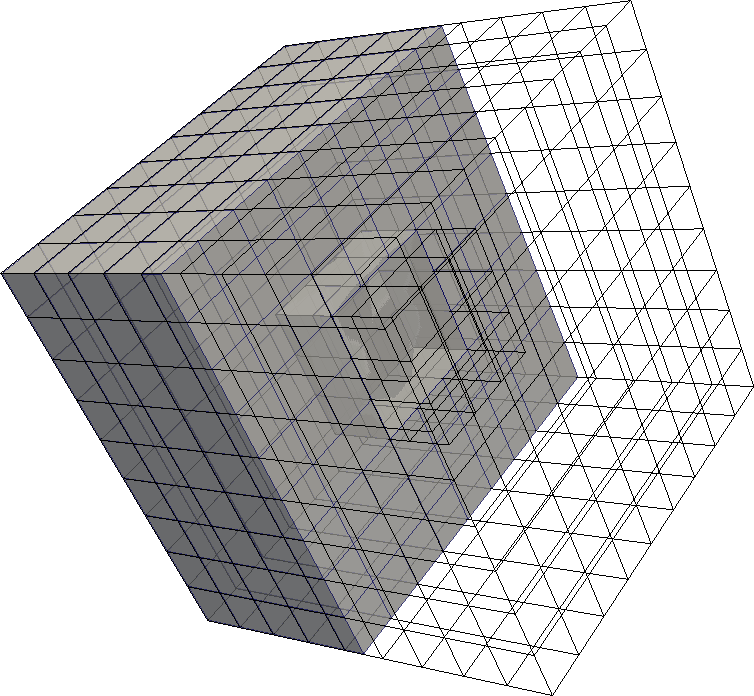
\includegraphics[width=0.55\textwidth]{2_quickstart/cube.png}
\end{center}


\section{A tree within the spacetree}

In the final example we create a slightly more interesting setup. 
We solely edit the operation \texttt{createInnerVertex} within the  
file \texttt{myproject/mappings/CreateGrid.cpp}, recompile it and 
have a look at the result.
When you study source code, please note the similarity to Matlab when we work
with vectors in Peano; as well as that the indices start with 0.
If your want to get rid of all the debug statements and are sick of long 
waiting times, remove the \texttt{-DDebug} statement in the line  
\texttt{PROJECT\_CFLAGS = -DDebug -DAsserts}
within the makefile.
There are more elegant ways to filter out log statements that we will discuss
later.


\begin{code}

void myproject::mappings::CreateGrid::createInnerVertex(
 myproject::Vertex&                          fineGridVertex,
 const tarch::la::Vector<DIMENSIONS,double>& fineGridX,
 const tarch::la::Vector<DIMENSIONS,double>& fineGridH,
 myproject::Vertex * const                   coarseGridVertices,
 const peano::grid::VertexEnumerator&      coarseGridVerticesEnumerator,
 myproject::Cell&                            coarseGridCell,
 const tarch::la::Vector<DIMENSIONS,int>&    fineGridPositionOfVertex 
) {
 logTraceInWith6Arguments("createInnerVertex(...)",fineGridVertex,...);
  
 if (
   fineGridVertex.getRefinementControl()==Vertex::Records::Unrefined 
   &&
   coarseGridVerticesEnumerator.getLevel()<4
 ) {
   bool trunk = (fineGridX(0)-0.5)*(fineGridX(0)-0.5)
              + (fineGridX(2)-0.5)*(fineGridX(2)-0.5)<0.008;
   bool treeTop = (fineGridX(0)-0.5)*(fineGridX(0)-0.5)
                + (fineGridX(1)-0.7)*(fineGridX(1)-0.7)
                + (fineGridX(2)-0.5)*(fineGridX(2)-0.5)<0.3*0.3;
   if (trunk | treeTop) {
     fineGridVertex.refine();
   }
 }

 logTraceOutWith1Argument("createInnerVertex(...)",fineGridVertex);
}
\end{code}

So here's what I get. Feel free to create better pics:

\begin{center}
  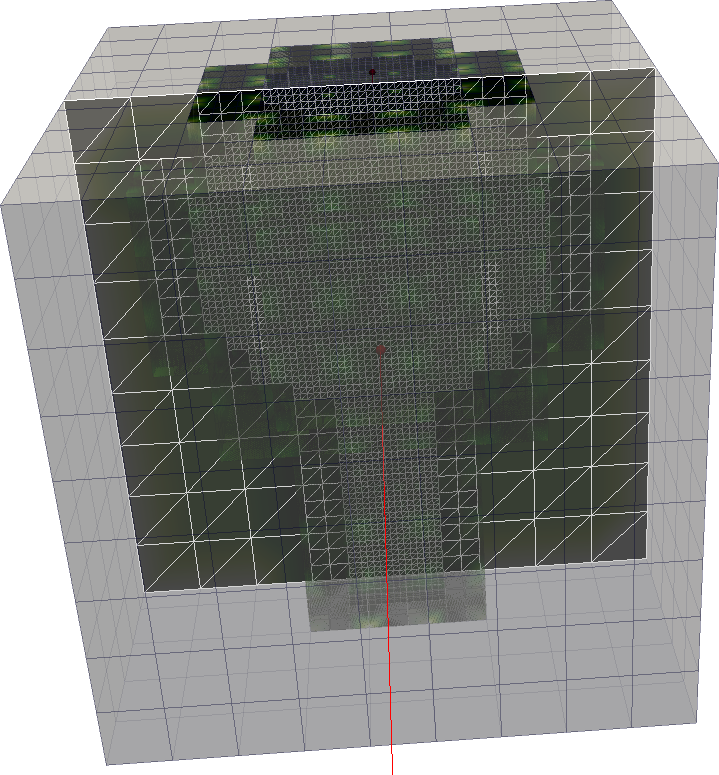
\includegraphics[width=0.55\textwidth]{2_quickstart/tree.png}
\end{center}

\subsection*{Further reading}

\begin{itemize}
  \item Weinzierl, Tobias and Mehl, Miriam (2011). {\em Peano---A Traversal and
  Storage Scheme for Octree-Like Adaptive Cartesian Multiscale Grids}. SIAM
  Journal on Scientific Computing 33(5): 2732-2760.
  \item Bungartz, Hans-Joachim, Eckhardt, Wolfgang, Weinzierl, Tobias and
  Zenger, Christoph (2010). {\em A Precompiler to Reduce the Memory Footprint of
  Multiscale PDE Solvers in C++}. Future Generation Computer Systems 26(1): 175-182.
  \item Bungartz, Hans-Joachim, Mehl, Miriam, Neckel, Tobias and Weinzierl,
  Tobias (2010). {\em The PDE framework Peano applied to fluid dynamics: an efficient
  implementation of a parallel multiscale fluid dynamics solver on octree-like adaptive Cartesian grids}. Computational Mechanics 46(1): 103-114.
  \item   Weinzierl, Tobias (2009). {\em A Framework for Parallel PDE Solvers on
  Multiscale Adaptive Cartesian Grids}. M\"unchen: Verlag Dr. Hut.
  \item Bungartz, Hans-Joachim, Mehl, Miriam, Weinzierl, Tobias and Eckhardt,
  Wolfgang (2008). {\em DaStGen---A Data Structure Generator for Parallel C++
  HPC Software}. In ICCS 2008: Advancing Science through Computation, Part III.
  Bubak, van Albada, Sloot and Dongarra, Heidelberg, Berlin: Springer-Verlag.
  5103: 213-222.
  \item Brenk, Markus, Bungartz, Hans-Joachim, Mehl, Miriam, Muntean, Ioan
  Lucian, Neckel, Tobias and Weinzierl, Tobias (2008). {\em Numerical Simulation
  of Particle Transport in a Drift Ratchet}. SIAM Journal of Scientific Computing 30(6): 2777-2798.
\end{itemize}
